% !TEX TS-program = pdflatex
\documentclass[15pt,aspectratio=169]{beamer}

% ------------------------------------------------------------------
% Theme & visual tweaks
% ------------------------------------------------------------------
\usetheme{metropolis}
\metroset{progressbar=frametitle}
\setbeamertemplate{frame numbering}[fraction] % 1/12 unten rechts
\definecolor{blockgray}{RGB}{225,225,225}  % ~20 % gray

% --------------------------------------------------------------
% Encoding & fonts
% --------------------------------------------------------------
\usepackage[utf8]{inputenc}
\usepackage[T1]{fontenc}
\usepackage{textcomp}
\usepackage{microtype}      % nicer text
\usepackage{pifont}
\usepackage{booktabs}
\usepackage{fontawesome5}   % icons, falls noch genutzt

% --------------------------------------------------------------
% TikZ & PGFPlots
% --------------------------------------------------------------
\usepackage{tikz,adjustbox}
\usetikzlibrary{positioning,arrows.meta,fit,calc,trees}
\usepackage{pgfplots}
\pgfplotsset{compat=newest,plot coordinates/math parser=false}

% --------------------------------------------------------------
% Maths & abbreviations
% --------------------------------------------------------------
\usepackage{amsmath,physics,xspace}
\newcommand{\tfidf}{TF-IDF\xspace}
\newcommand{\TFIDF}{Term-Frequency-Inverse-Document-Frequency\xspace}
\newcommand{\IForest}{Isolation Forest\xspace}
\newcommand{\RForest}{Random Forest\xspace}
\newcommand{\LOC}{lines of code\xspace}

% --------------------------------------------------------------
% TikZ box styles
% --------------------------------------------------------------
\tikzset{
  box/.style = {rectangle, draw, rounded corners=3pt,
                text width = 4.6cm, align = center,
                minimum height = 1.05cm,
                font = \small, fill = blockgray},
  side/.style = {box, text width = 3.8cm, fill = blue!7},
  arr/.style  = {-{Stealth[length=3mm,width=2mm]}, thick},
  lab/.style  = {font=\scriptsize, sloped, anchor=south, midway}
}

% --------------------------------------------------------------
% Meta data
% --------------------------------------------------------------
\title{Use of AI for Log Analysis in CI/CD Pipelines}
\subtitle{Bachelor Thesis -- Defence}
\author{Maid Ališi\'c}
\institute{%
  FH Oberösterreich · Campus Hagenberg\\[1ex]
  Supervisor: FH‑Prof.\ Dipl.‑Ing.\ Dr.\ Stefan Wagner
}
\date{July 23, 2025}

% ==============================================================
\begin{document}
% ==============================================================

% ----------------------------------------------------------------
% Title slide
% ----------------------------------------------------------------
\maketitle

% ----------------------------------------------------------------
% Agenda slide
% ----------------------------------------------------------------
\begin{frame}{Road map}
  \tableofcontents[hideallsubsections]
\end{frame}

% ================================================================
\section{Research questions}
% ================================================================

\begin{frame}{Research questions}
  \centering
  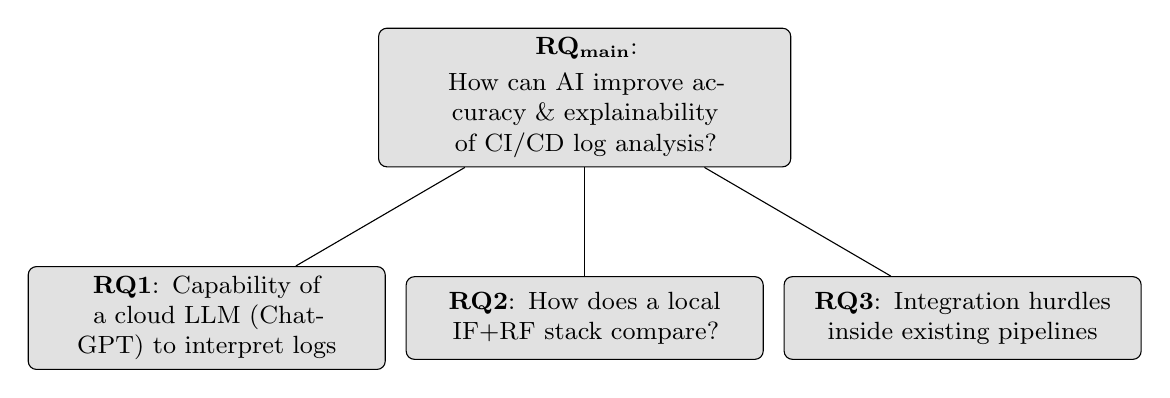
\begin{tikzpicture}[
      grow=down,
      level distance=2.8cm,
      level 1/.style={sibling distance=4.8cm},
      box/.style = {rectangle, draw, rounded corners=3pt,
                    text width = 4.6cm, align = center,
                    minimum height = 1.05cm,
                    font = \small, fill = blockgray}
    ]
    \node[box,text width=5cm] (main)
      {\textbf{RQ\textsubscript{main}}:\\[2pt]
       How can AI improve accuracy \& explainability\\
       of CI/CD log analysis?}
      child { node[box,text width=4.3cm]
        {\textbf{RQ1}: Capability of a cloud LLM (ChatGPT) to interpret logs} }
      child { node[box,text width=4.3cm]
        {\textbf{RQ2}: How does a local IF+RF stack compare?} }
      child { node[box,text width=4.3cm]
        {\textbf{RQ3}: Integration hurdles inside existing pipelines} };
  \end{tikzpicture}
\end{frame}

% ================================================================
\section{Problem context}
% ================================================================

\begin{frame}{Why do we care?}
\begin{itemize}[<+->]
  \item CI/CD emits \alert{$\approx$ 10--20 GB} of build, test \& deploy logs \textit{per day}.
  \item Manual \texttt{grep} slows the merge queue; critical faults slip through.
  \item Business \textbf{Service-Level Objective}: feedback within \alert{$\le 200$ ms} per pipeline.
  \item Logs may expose customer IDs, therefore they must remain on-premises (no cloud export).
\end{itemize}
\end{frame}

\begin{frame}{Operational pain points}
\begin{enumerate}[<+->]
  \item \textbf{Context-sensitivity} -- identical tokens can be harmless or fatal.
  \item \textbf{Concept drift} -- each merge may rename tests or switches.
  \item \textbf{Latency pressure} -- analysis must finish before the job completes.
  \item \textbf{Alert fatigue} -- regex rule sets grow without bound.
\end{enumerate}
\end{frame}

% ================================================================
\section{Method}
% ================================================================

\subsection{Feature engineering}
\begin{frame}{Vectorisation pipeline \ding{172}}
\begin{columns}
  \column{.55\linewidth}
    \begin{enumerate}[<+->]
      \item \textbf{Normalise} -- strip timestamps, colours, IDs.
      \item \textbf{Tokenise} into uni- and bi-grams.
      \item Weight with \tfidf.
      \item Produce sparse vector.
    \end{enumerate}
  \column{.45\linewidth}
    \centering
    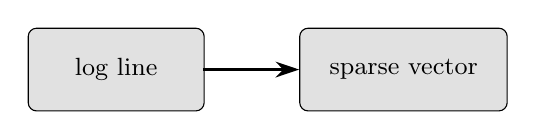
\begin{tikzpicture}[node distance=1.1cm]
      \node[box,text width=2cm]{log line};
      \node[box,right=1.2cm of {$(current bounding box.east)!0.5!(current bounding box.east)$},text width=2.4cm] (vec){sparse vector};
      \draw[arr] (1.1,0) -- (vec.west);
    \end{tikzpicture}
\end{columns}
\end{frame}

\subsection{Algorithms}
\begin{frame}{Isolation Forest \ding{173} -- intuition}
\begin{columns}
  \column{.55\linewidth}
  \begin{itemize}[<+->]
    \item Random binary partitioning isolates unusual lines in fewer splits.
    \item Score \(s(x)=2^{-h(x)/c(n)} \in [0,1]\); high $\Rightarrow$ outlier.
    \item CPU-only: \(\approx 30\,\mu s\) per line.
  \end{itemize}
  \column{.45\linewidth}
    \centering
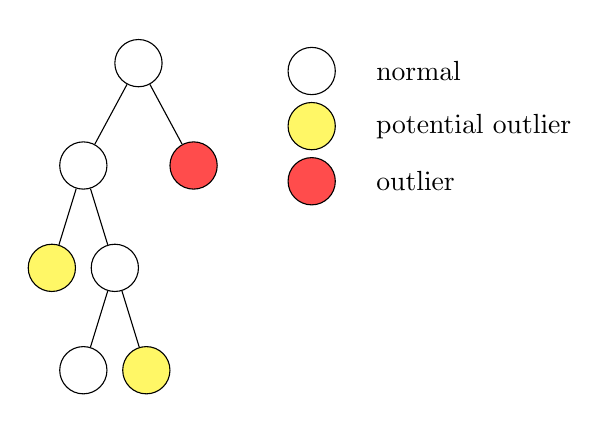
\begin{tikzpicture}[
  level distance = 1.3cm,
  level 1/.style={sibling distance=1.4cm},
  level 2/.style={sibling distance=0.8cm},
  every node/.style={circle, draw, minimum size=6mm, inner sep=0pt},
  normal/.style  ={fill=white!10},
  potout/.style  ={fill=yellow!60},
  outlier/.style ={fill=red!70},
  empty/.style   ={fill=white}
]
  \node[empty] {}
    child {node[empty] {}
      child {node[potout] {}}
      child {node[empty] {}
        child {node[empty] {}}
        child {node[potout] {}}
      }
    }
    child {node[outlier] {}};

  % Legend
  \begin{scope}[xshift=2.2cm, yshift=-0.1cm]
    \node[circle,draw,minimum size=6mm,inner sep=0pt,normal]  at (0,0)    {};
    \node[circle,draw,minimum size=6mm,inner sep=0pt,potout]  at (0,-0.7) {};
    \node[circle,draw,minimum size=6mm,inner sep=0pt,outlier] at (0,-1.4) {};
    \node[anchor=west,draw=none] at (0.8,  0)   {normal};
    \node[anchor=west,draw=none] at (0.8,-0.7) {potential outlier};
    \node[anchor=west,draw=none] at (0.8,-1.4) {outlier};
  \end{scope}
\end{tikzpicture}
\end{columns}
\end{frame}

\begin{frame}{Random Forest \ding{174} -- error labelling}
\begin{columns}
  \column{.55\linewidth}
  \begin{itemize}[<+->]
    \item Maps each flagged line to a domain-specific error category.
    \item Majority vote $\Rightarrow$ deterministic, auditable output.
    \item Nightly retrain $<$ 90 s; warm-start handles drift.
  \end{itemize}
  \column{.45\linewidth}
    \centering
    \begin{adjustbox}{max width=.85\linewidth}
      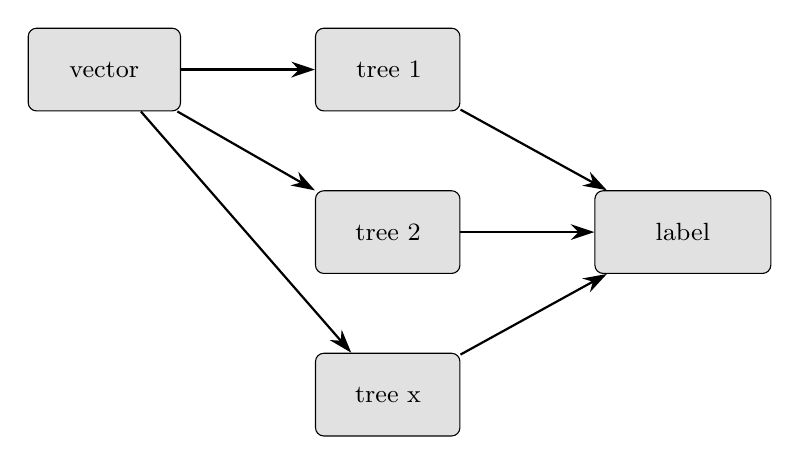
\begin{tikzpicture}[node distance=1cm]
        \node[box,text width=1.7cm] (v){vector};
        \node[box,right=1.7cm of v,text width=1.6cm] (t1){tree 1};
        \node[box,below=of t1,text width=1.6cm] (t2){tree 2};
        \node[box,below=of t2,text width=1.6cm] (t3){tree x};
        \node[box,right=1.7cm of t2,text width=2cm] (vote){label};
        \draw[arr](v)--(t1);
        \draw[arr](v)--(t2);
        \draw[arr](v)--(t3);
        \draw[arr](t1)--(vote);
        \draw[arr](t2)--(vote);
        \draw[arr](t3)--(vote);
      \end{tikzpicture}
    \end{adjustbox}
\end{columns}
\end{frame}

% ================================================================
\section{Architecture}
% ================================================================

\begin{frame}{End-to-end pipeline ($< 40$ ms inline)}
\centering
\begin{adjustbox}{max width=.98\linewidth,max height=.9\textheight}
  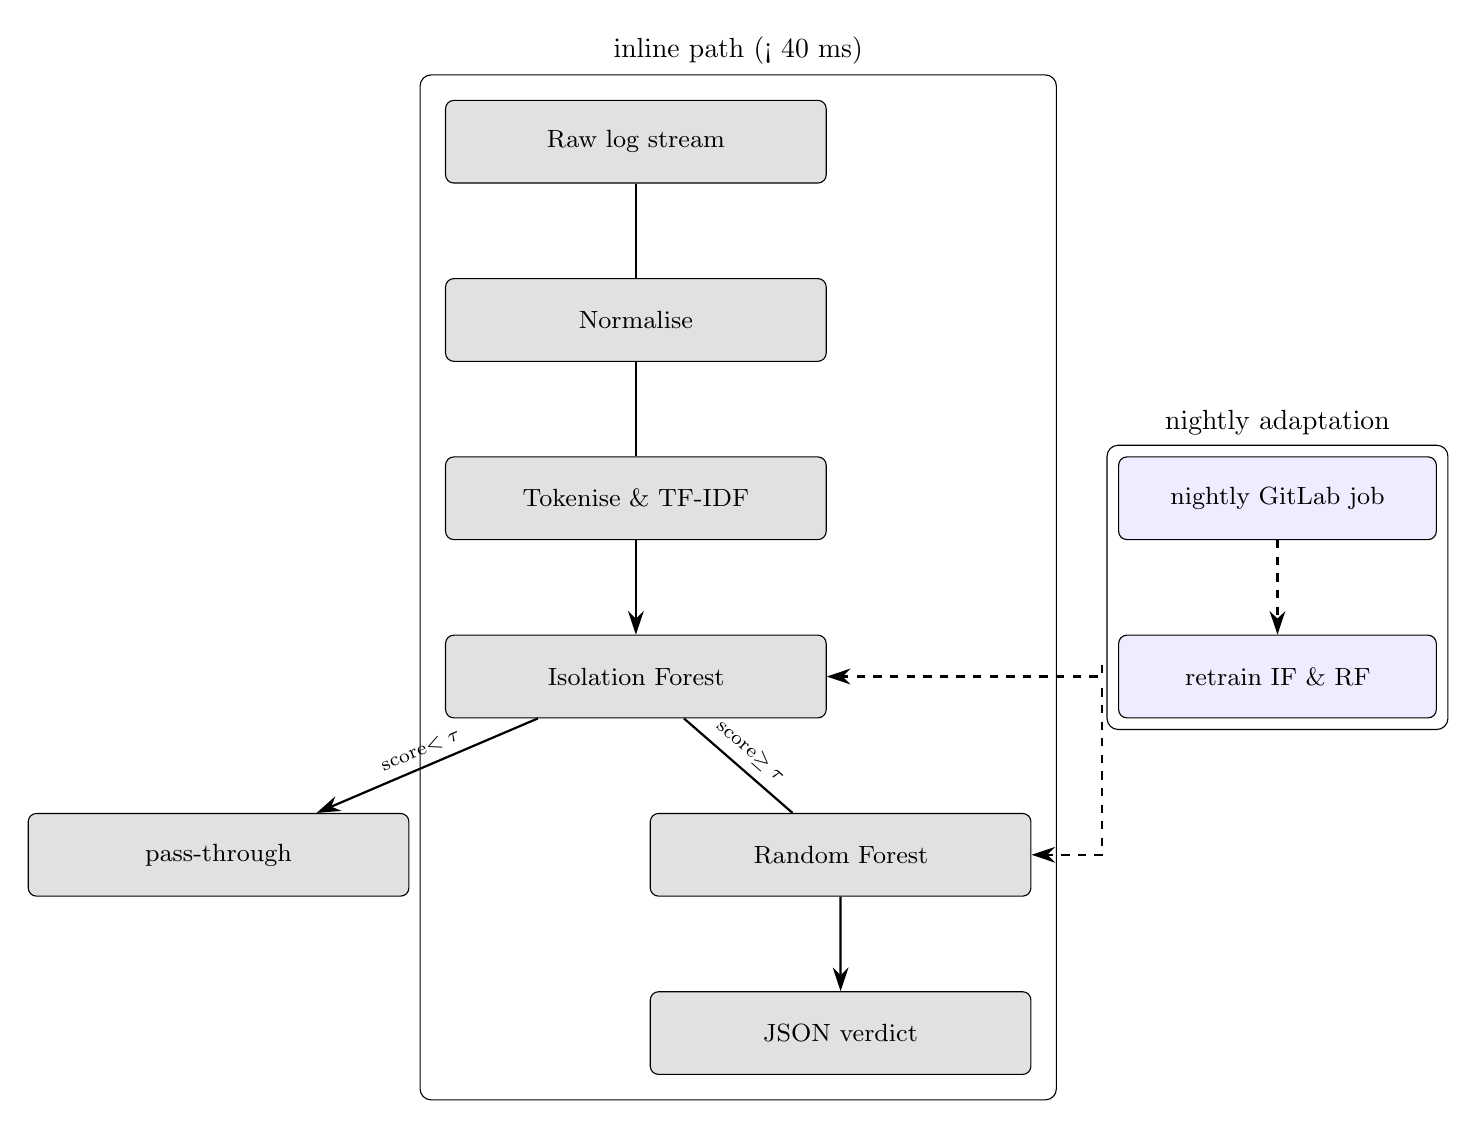
\begin{tikzpicture}[node distance=1.2cm and 1.8cm]
    \node[box] (raw){Raw log stream};
    \node[box,below=of raw] (norm){Normalise};
    \node[box,below=of norm] (vect){Tokenise \& TF-IDF};
    \node[box,below=of vect] (ifor){\IForest};
    \node[box,below=of ifor,xshift=+2.6cm] (rfor){\RForest};
    \node[box,below=of rfor] (json){JSON verdict};
    \node[box,below=of ifor,xshift=-5.3cm] (pass){pass-through};
    \draw[arr] (raw)--(norm)--(vect)--(ifor);
    \draw[arr] (ifor)--node[lab]{score$<\tau$}(pass);
    \draw[arr] (ifor)--node[lab]{score$\ge\tau$}(rfor)--(json);
    \node[side,right=3.7cm of vect] (cron){nightly GitLab job};
    \node[side,below=of cron] (train){retrain IF \& RF};
    \draw[arr,dashed] (cron)--(train);
    \draw[arr,dashed] (train.west)+(-.2,.15)|-(ifor.east);
    \draw[arr,dashed] (train.west)+(-.2,-.15)|-(rfor.east);
    \node[draw,rounded corners=4pt,inner sep=9pt,fit=(raw)(json),label=above:{inline path (< 40 ms)}]{};
    \node[draw,rounded corners=4pt,inner sep=4pt,fit=(cron)(train),label=above:{nightly adaptation}]{};
  \end{tikzpicture}
\end{adjustbox}
\end{frame}

% ================================================================
\section{Data \& evaluation}
% ================================================================

\begin{frame}{Datasets \& metrics}
\begin{columns}
  \column{.55\linewidth}
  \begin{itemize}[<+->]
     \item 117 k \textit{macOS} logs + 655 k \textit{OpenSSH} logs
     \item 504 labelled anomalies (class imbalance $\approx$ 1 : 200)
     \item Split 70 / 15 / 15 \% (training / validation / testing)
     \item Metrics: Precision, Recall and $F_{1}$
  \end{itemize}
  \column{.45\linewidth}
    \centering
    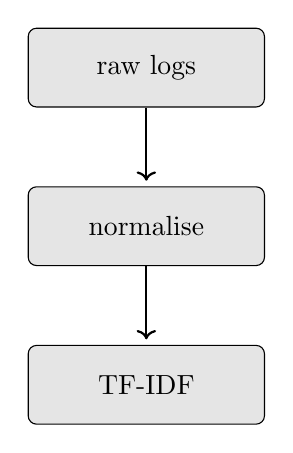
\begin{tikzpicture}[node distance=1cm,
      box/.style={
        draw, rounded corners=3pt, fill=gray!20,
        minimum width=3cm, minimum height=1cm, align=center},
      arr/.style={->, thick, shorten >=2pt}
    ]
    \node[box] (raw)  {raw logs};
    \node[box, below=of raw]  (norm) {normalise};
    \node[box, below=of norm] (vec) {TF-IDF};
    \draw[arr] (raw.south) -- (norm.north);
    \draw[arr] (norm.south) -- (vec.north);
  \end{tikzpicture}
\end{columns}
\end{frame}

% ================================================================
\section{Results}
% ================================================================

\begin{frame}{Headline numbers}
\centering
\begin{tabular}{lccc}
  \toprule
   & Precision & Recall & $F_{1}$ \\
  \midrule
  Detection (\IForest)        & 0.91 & 0.88 & 0.89 \\
  Classification (\RForest)   & 0.99 & 0.99 & 0.99 \\
  \addlinespace
  Regex baseline              & 0.286 & 0.286 & 0.286 \\
  \bottomrule
\end{tabular}

\vspace{.8em}
\small
$F_{1} = 2 \cdot \dfrac{P \cdot R}{P + R}$
\end{frame}

% ================================================================
\section{Impact}
% ================================================================

\begin{frame}{Operational impact}
\begin{itemize}[<+->]
  \item \textbf{Latency}: minutes $\rightarrow$ \textbf{milliseconds} (inline verdict).
  \item \textbf{Cost-free}: 2.3 k \LOC{}, CPU-only, no token fees.
  \item \textbf{GDPR compliant}: logs never leave the VPN.
\end{itemize}
\end{frame}

% ================================================================
\section{Wrap-up}
% ================================================================

\begin{frame}{Take-away}
\vspace{2em}
\centering
{\Large
  \textbf{Light-weight on-prem ML matches AIOps SaaS}\par
  \vspace{.4em}
  without latency, cost or privacy pain.
}

\vspace{2.2em}
\small
Questions welcome -- thank you!
\end{frame}

\end{document}
